% This is "sig-alternate.tex" V2.0 May 2012
% This file should be compiled with V2.5 of "sig-alternate.cls" May 2012
%
% This example file demonstrates the use of the 'sig-alternate.cls'
% V2.5 LaTeX2e document class file. It is for those submitting
% articles to ACM Conference Proceedings WHO DO NOT WISH TO
% STRICTLY ADHERE TO THE SIGS (PUBS-BOARD-ENDORSED) STYLE.
% The 'sig-alternate.cls' file will produce a similar-looking,
% albeit, 'tighter' paper resulting in, invariably, fewer pages.
%
% ----------------------------------------------------------------------------------------------------------------
% This .tex file (and associated .cls V2.5) produces:
%       1) The Permission Statement
%       2) The Conference (location) Info information
%       3) The Copyright Line with ACM data
%       4) NO page numbers
%
% as against the acm_proc_article-sp.cls file which
% DOES NOT produce 1) thru' 3) above.
%
% Using 'sig-alternate.cls' you have control, however, from within
% the source .tex file, over both the CopyrightYear
% (defaulted to 200X) and the ACM Copyright Data
% (defaulted to X-XXXXX-XX-X/XX/XX).
% e.g.
% \CopyrightYear{2007} will cause 2007 to appear in the copyright line.
% \crdata{0-12345-67-8/90/12} will cause 0-12345-67-8/90/12 to appear in the copyright line.
%
% ---------------------------------------------------------------------------------------------------------------
% This .tex source is an example which *does* use
% the .bib file (from which the .bbl file % is produced).
% REMEMBER HOWEVER: After having produced the .bbl file,
% and prior to final submission, you *NEED* to 'insert'
% your .bbl file into your source .tex file so as to provide
% ONE 'self-contained' source file.
%
% ================= IF YOU HAVE QUESTIONS =======================
% Questions regarding the SIGS styles, SIGS policies and
% procedures, Conferences etc. should be sent to
% Adrienne Griscti (griscti@acm.org)
%
% Technical questions _only_ to
% Gerald Murray (murray@hq.acm.org)
% ===============================================================
%
% For tracking purposes - this is V2.0 - May 2012

\documentclass[conference]{IEEEtran}
% ===============================================================
%    My Commands
    \newcommand{\bi}{\begin{itemize}}
    \newcommand{\ei}{\end{itemize}}
    \newcommand{\be}{\begin{enumerate}}
    \newcommand{\ee}{\end{enumerate}}
    \newcommand{\ii}{\item}
    \newtheorem{Def}{Definition}
    \newtheorem{Lem}{Lemma}

    \usepackage{algorithm}
    \usepackage{algorithmicx}
    \usepackage{algpseudocode}
%    \usepackage[lined,boxed,commentsnumbered]{algorithm2e}

    \usepackage{graphicx}
    \graphicspath{%
        {converted_graphics/}% inserted by PCTeX
        {./images/}% inserted by PCTeX
    }

\usepackage{times}
% ===============================================================

\begin{document}
    %
    % paper title
    % can use linebreaks \\ within to get better formatting as desired
    \title{A Collaboration Middleware for Peer-to-Peer Architecture}

    % author names and affiliations
    % use a multiple column layout for up to three different
    % affiliations
    \author{\IEEEauthorblockN{Sung-Soo Kim, Chunglae Cho and Jongho Won}
    \IEEEauthorblockA{
            Electronics and Telecommunications Research Institute (ETRI)\\
            Daejeon, South Korea \\
            {\it \{sungsoo, clcho, jhwon\}@etri.re.kr}
    }
    }


\maketitle
\begin{abstract}
We introduce a novel mobile middleware which provides a collaboration service among associated apps in a symmetric fashion.
This paper focuses on the challenge that how users can  receive the seamless collaboration services regardless of the changes of physical device configurations in the multiscreen environment.
In order to solve this problem, we propose a novel system architecture which supports primitive operations, such as remote invocation, session join/invitation,  push/pull migration and synchronization for collaboration among associated applications.

The major advantages of our system are that the system can provides communication transparency, seamless collaboration services and scalability.
The experimental results demonstrate that our system can be successfully applied to the collaboration services among multiple apps in the small network.
\end{abstract}

% A category with the (minimum) three required fields
    \begin{IEEEkeywords}
Mobile Middleware, Collaboration Session
    \end{IEEEkeywords}

\section{Introduction}
In the fields of broadcasting especially IPTV and content delivery, multiscreen video describes video content transformed into multiple formats, bit rates and resolutions for display on smart devices such as television, mobile phone, tablet computer and computer \cite{Lucent2011}.
However, previous methods related to multiscreen IPTV focused on transcoding the multimedia for adaptive content delivery. 
In recent years, there has been an increased interest in smart applications (or \textit{apps}) running on various smart devices, such as smartphones and tablets. 
The main reason for this has been the realization that many diverse apps need a dedicated middleware for managing apps and collaborating among multiple associated apps 
\cite{
samsung:2014, 			% 1
Aarts:2004, 			% 2
Anstead:2014, 			% 3
Barkhuus:2009, 			% 4
DBLP:FuentesPCM06, 	% 5	
Longo:2013, 			% 6
Lucent2011,			% 7
Ma:2008,				% 8
Motti:2013,			% 9	
Nandakumar:2014, 		% 10
Sadri:2011, 			% 11
DBLP:SchmohlB08}. 		% 12

A second screen is a second smart device used by television viewers to connect to a program they're watching. 
A second screen is often a smartphone or tablet, where a special complementary app may allow the viewer to interact with a television program in a different way -- the tablet or smartphone becomes a TV companion device. Prior research has focused on achieving 

%In this paper, we introduce a novel mobile middleware which can support the collaboration services among multiple associated apps. 
%A Smart Home environment is a home equipped with sensors and activators of various types to monitor activities and movement, and to monitor risk situations, such as fire and smoke alarms. 
%
% Reference paper: Heterogeneity in mobile computing environments
%The goal of mobile computing suggests including devices spanning the entire hardware spectrum. 
%This augmentation includes the \textit{Internet of Things} (IoT) appliance of various use cases,  including both the pervasive access to mobile services and ubiquitous communication between smart devices. Hence, those application cases can be reduced to the basic demand of communication among heterogenous devices in heterogenous environment.
%The ultimate goal of mobile middleware is to simplify the development of distributed applications.
%The goal of mobile middleware is to provide abstractions that reduce development effort, to offer programming paradigms that make developing powerful mobile applications easier, and to foster interoperability between applications.
%The essential role of middleware is to manage the complexity and heterogeneity of distributed infrastructures. 
%On the one hand, middleware offers programming abstractions that hide some of the complexities of building a distributed application.
%On the other hand, there is a complex software infrastructure that implements these abstractions.
%Middleware is software that supports mediation between other software components, fostering interoperability between those components across heterogeneous platforms and varying resource levels.
%Mobile agents put the action where the data are, allowing programs to move autonomously about a network in order to access remote resources.
%
%Service discovery middleware extends the client-server paradigm to include dynamic discovery of services and more dynamic interaction between clients and services.
%With service discovery middleware, developers can quickly develop highly dynamic client-server systems that are self-healing and support "plug and play" for individual components.
%The concepts embodied in service discovery architectures are not completely new; however, service discovery frameworks standardize the environments in which to deploy highly dynamic, self-healing client-server architectures.
%
%In the fields of broadcasting especially IPTV and content delivery, multiscreen video describes video content transformed into multiple formats, bit rates and resolutions for display on smart devices such as television, mobile phone, tablet computer and computer.
%
% %Reference paper: Ambient Intelligence: A Multimedia Perspective
%The complexity of media will continually increase in terms of volume and functionality, thus introducing a need for simplicity and ease of use. Therefore, the massively distributed, integrated use of media will require replacing well-known interaction vehicles, such as remote control and menu driven search and control, with novel, more intuitive, and natural concepts.
%
%Ambient intelligence aims to take the integration provided by ubiquitous computing one step further by realizing environments that are sensitive and responsive to the presence of people. The focus is on users and their experiences from a consumer-electronics perspective.
%
%The new paradigm aims to improve people's quality of life by creating the desired atmosphere and functionality through intelligent, personalized, interconnected systems and services. The term ambient refers to the environment and reflects the need for typical requirements such as distribution, ubiquity, and transparency. \textit{Distribution} refers to noncentral systems control and computation. \textit{Ubiquity} means the embedding is present everywhere. \textit{Transparency} indicates that the surrounding systems are invisible and unobtrusive. \textit{Intelligence} means the digital surrounding exhibit specific forms of social interaction. In other words, and environment must recognize the people that live in it, adapt itself to them, learn from their behavior, and possibly show emotion. 
%\noindent
%\textbf{Key features of ambient intelligence: }
%To refine the notion of ambient intelligence, Morzano et. al. formulated the following five key technology features.
%such as embedded, context-aware, personalized, adaptive and  anticipatory.
In this paper, we propose a novel mobile middleware to support the seamless collaboration services among heterogenous multiple apps in diverse smart devices.
To provide convincing the collaboration services in multiscreen environments, we describe the key requirements 
%of collaboration service systems 
as follows:
\bi
\ii \emph{Service Discovery}: 
Since the wireless hosts in the wireless network are highly dynamic,  service hosts should periodically announce their presence in the network.
Service discovery is one of the most important functions in order to collaborate among apps through remote invocation and session join/invitation in mobile computing environments.
\ii \emph{Collaboration}: 
The system must support  collaboration services among apps in smart devices. To satisfy this requirement, the system allows apps to join or leave a \textit{collaboration session} which is a logical space being synchronized via associated information at runtime.
However, collaboration session management in a peer-to-peer environment is quite challenging since its dynamic property. 
 \ii \emph{Mobility}: 
The system must support \textit{app migration} function, which migrates certain running apps from arbitrary device to other device at runtime.
\ii \emph{Scalability}: 
The system must be able to scale with the growth in the number of apps for collaboration services. For example, it must support the dynamic session joins for new apps during a certain collaboration service is provided. So, it is necessary to develop the collaboration session management techniques to provide the service scalability.
\ei

%\noindent
%\textbf{Motivation:} In this paper, .....

\noindent
\textbf{Our contributions:} We present a novel system architecture for the multiscreen-based collaboration services, which utilizes the collaboration middleware for multiple associated apps in the same wireless network and the remote service cloud. The contributions of our work can be summarized as follows.
\bi
\ii \textit{Collaboration middleware}: 
Our proposed middleware, which is based on peer-to-peer communication model, provides common APIs for diverse collaboration-based applications. Our middleware APIs include the primitive functions, such as, remote execution, session join/invitation and app migration.
\ii \textit{Service scalability}: 
We introduce a schema for representing inter-app relationship in collaboration sessions. This model can help design collaboration services and add additional apps for service extension. 
\ii \textit{Lifecyle managment}: We propose a method for logical app lifecycle management  to  support seamless collaboration session.
\ei

The rest of the paper is organized as follows.
Section \ref{sc:Architecture} describes the proposed the system architecture and the core components in our system.
We briefly survey previous work on multiscreen middleware, multiscreen IPTV, and second screen in Section \ref{sc:RelatedWork}.
In Section \ref{sc:Experiments}, we  presents the experimental results of our work in terms of service discovery.
Finally, we discuss future work and conclude in Section \ref{sc:Conclusion}.

%\section{Related Work}
%\label{sc:RelatedWork}
%In this section, we give a brief overview of related work on the middleware for mobile computing and multiscreen services.
%    We also highlight many technical characteristics of multiscreen user experience technology.\\
%
%Many researchers agree in handling heterogeneity by employing middleware solutions.
%The key idea behind the middleware approaches is to position the middleware layer between the application layer at the top and the heterogeneous environments such as hardware and operating systems at the bottom. 

\section{System Architecture}
    \label{sc:Architecture}
    In this section, we describe the proposed system architecture for the multiscreen-based collaboration services.
    Our architecture consists of two major systems such as the proposed middleware for smart devices and $n$-screen service cloud as shown in Fig. \ref{fig:architecture}. More specifically, our middleware decomposes into 2 layers;  the $n$-screen application library (NSAL) and the collaboration agent (CA).  

\subsection{System Overview}
%Figure \ref{fig:basicmodel} shows a high-level architectural view of our system utilizing cloud resources to provide the collaboration services among the associated applications.
Basically, our system architecture divided into two major systems as shown in Figure  \ref{fig:basicmodel}. 
First, our proposed architecture based on the \textit{Smart Home} concept is targeted at the smart home environment in terms of \textit{communication} and \textit{socialization}. 
    \begin{figure}[htb] % float placement: (h)ere, page (t)op, page (b)ottom, other (p)age
    \centering
    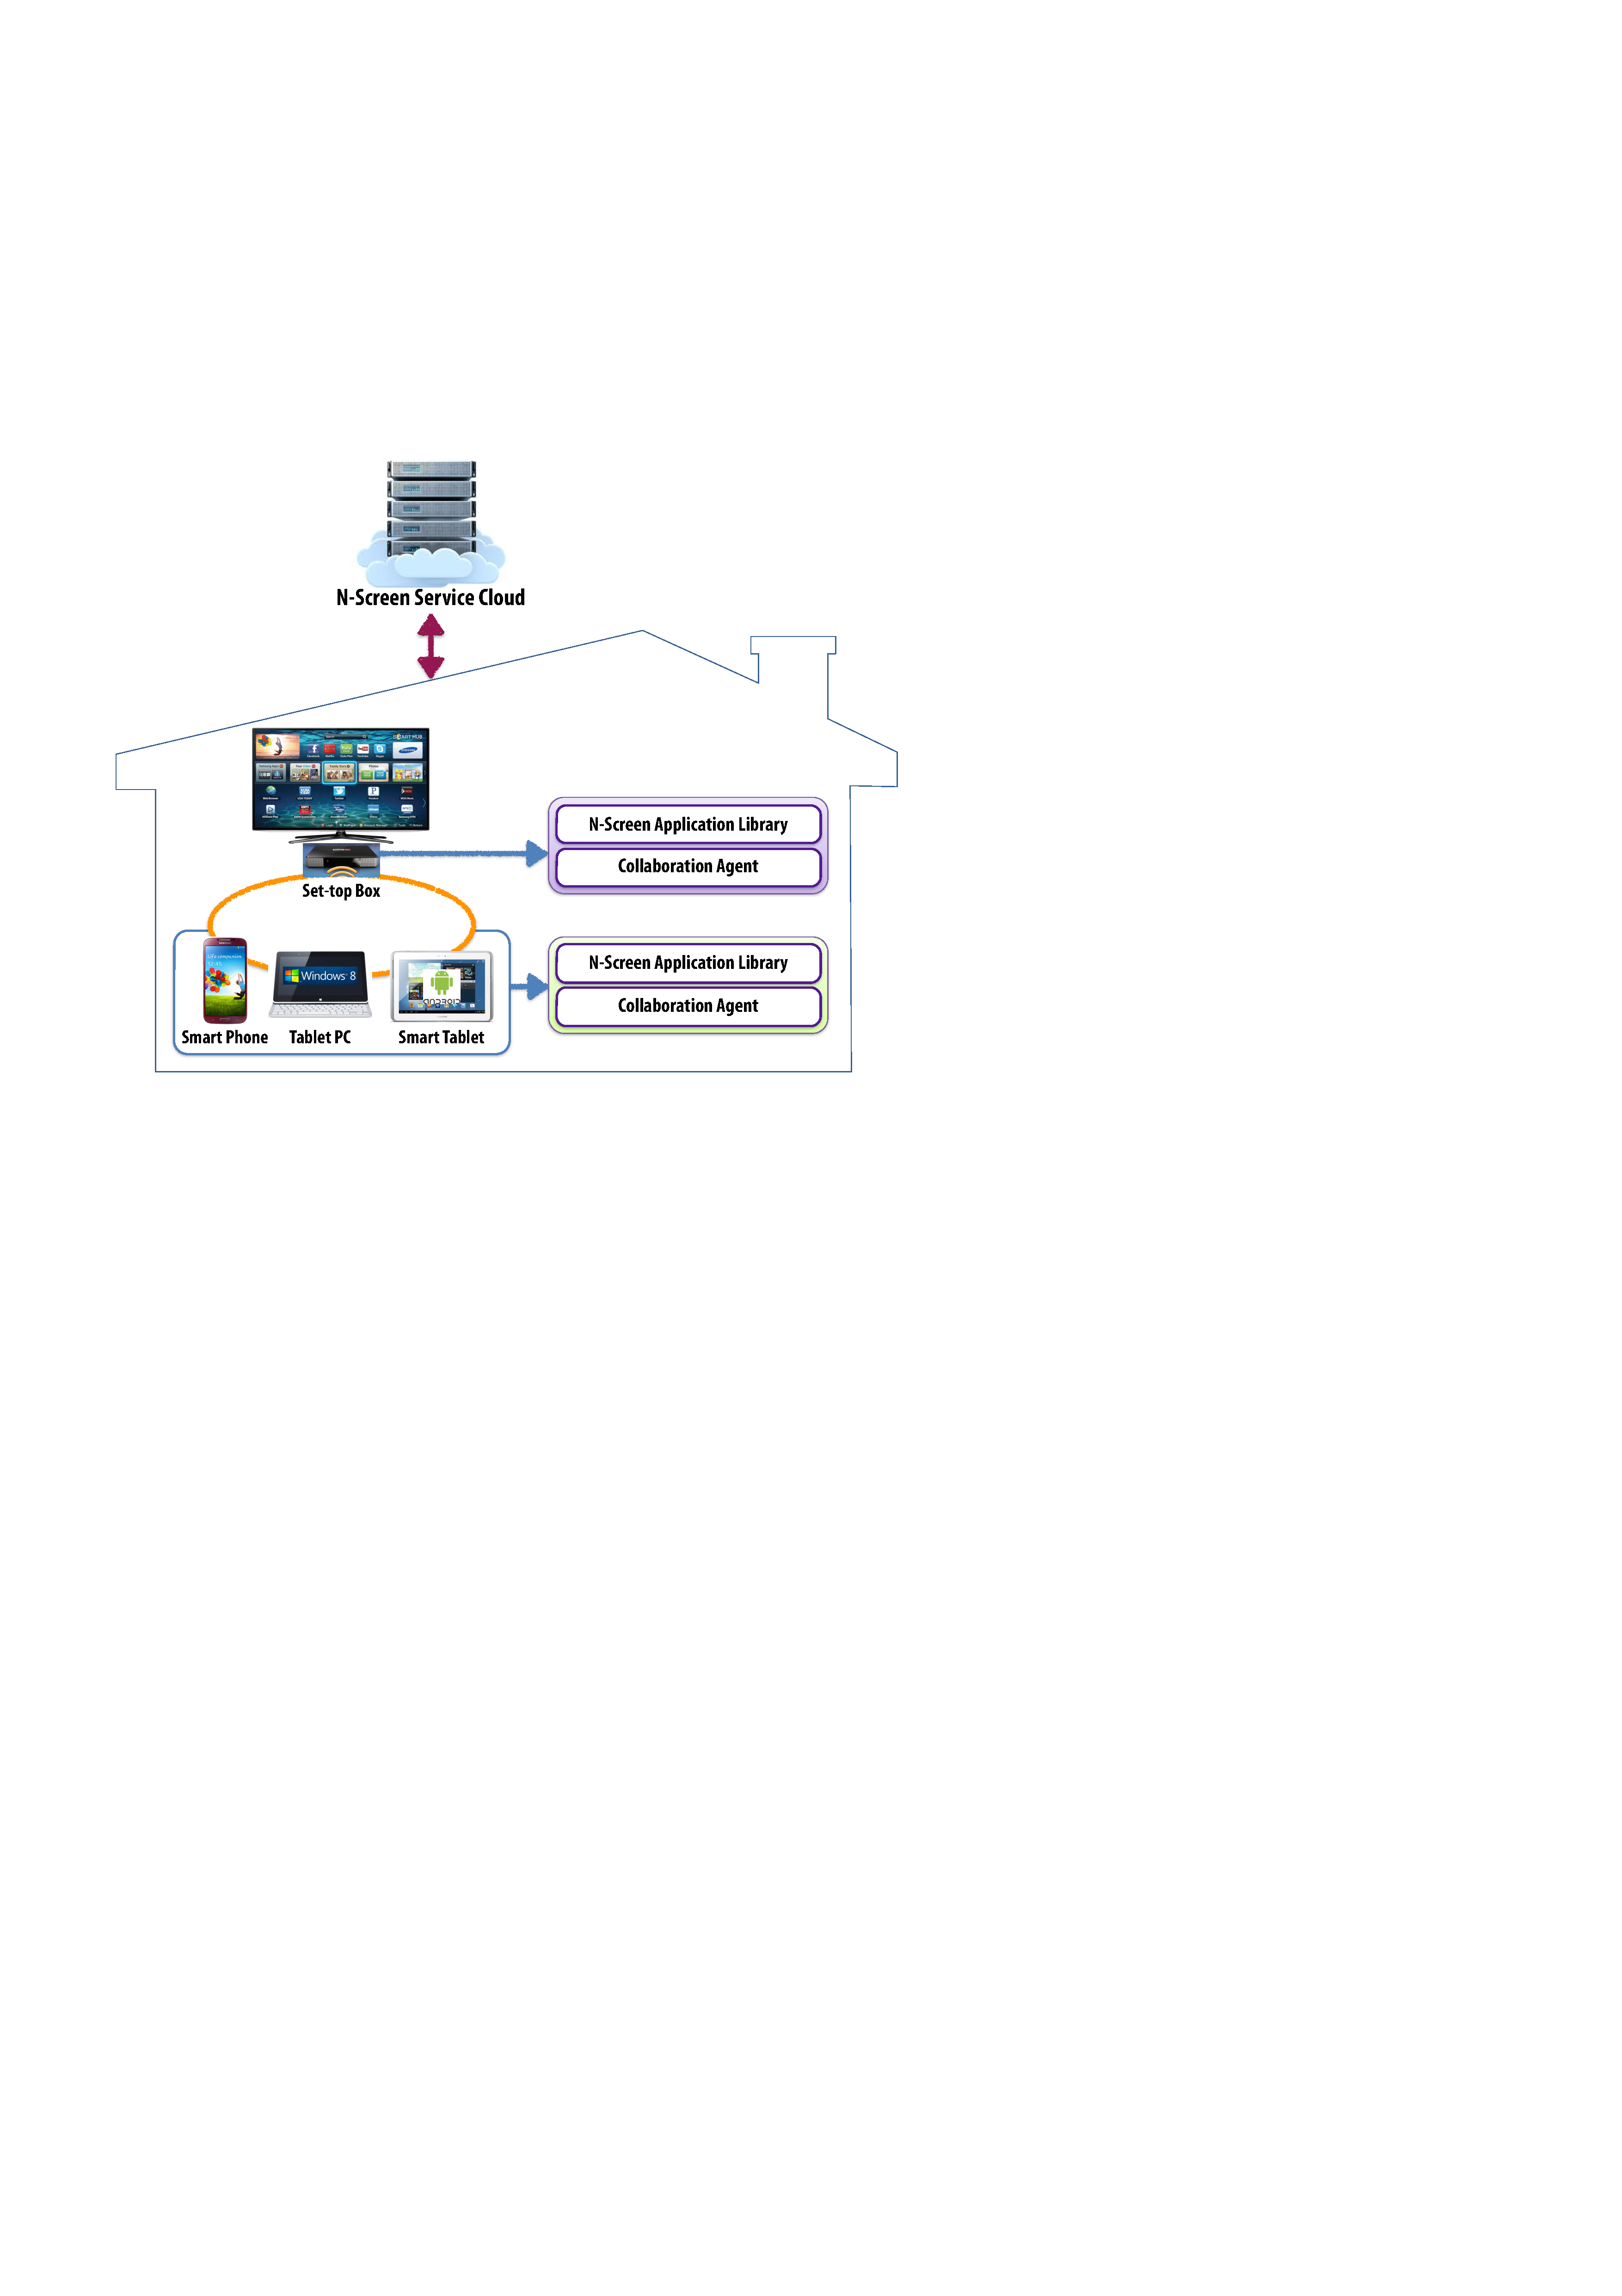
\includegraphics[width=8.5cm,keepaspectratio]{systemarchitecture}
    \caption{Our system architecture}
    \label{fig:architecture}
    \end{figure}

In our work, the smart home consists of various wireless hosts such as smartphone, smart set-top, smart tablet, or laptop which connects each other through a wireless communication link in the same wireless network environment. Each wireless host has the \textit{$n$-screen application library} and \textit{collaboration agent}, which provide abstractions that reduce development effort and support interoperability between applications. These mobile devices communicate directly with each other in a \textit{peer-to-peer} fashion with no centralized control.  Hence, the \textit{synchronization} for collaboration services is achieved through direct communication between applications.

Second,  the $n$-screen service cloud is responsible for providing the collaboration applications similar to the apps in the \textit{App Store} and managing the application contexts  for users. 
The primary benefit from the N-screen service cloud is \textit{scalability}, \textit{persistency} and \textit{mobility} for the collaboration service. 
 To represent the context of the application, we use the \textit{key-value pair} which is the most simple context model. Context information of the applications and collaboration sessions are stored in the context repository at the service cloud.


%Mobile devices communicate directly with each other in a peer-to-peer fashion with no centralized control.
%The peer-to-peer systems are distributed systems with no centralized control. The \textit{synchronization} for collaboration services is achieved through direct communication between applications.

%The goal of mobile middleware is to provide abstractions that reduce development effort, to offer programming paradigms that make developing a collaboration applications easier, and to support interoperability between applications.
%\subsection{Definitions}
% Formal definitions and notations
%There are several challenges that need to be addressed to support the collaboration services in multiscreen environments. 
    \begin{figure}[htb] % float placement: (h)ere, page (t)op, page (b)ottom, other (p)age
    \centering
    \includegraphics[width=6cm,keepaspectratio]{basicmodel}
    \caption{An example of $n$-screen collaboration service}
    \label{fig:basicmodel}
    \end{figure}

%We now briefly outline how the above challenges were addressed. 
%We now briefly define 

Here, we define major terminologies for our system architecture. The $n$-screen device $ND$ is a wireless host which includes the NSAL and the collaboration agent as shown in Fig. \ref{fig:basicmodel}.  Every $ND$ in the same network periodically sends UDP-based broadcast message for advertisement of their aliveness.\\

\noindent
\textbf{N-Screen-based Applications: }
There are two kinds of application; \textit{physical} and \textit{logical} applications (or \textit{app}).
First, the \textit{physical application}, $A_p$ is an application running on each device in the same network.  
This lifecycle of  $A_p$ is the same as the android application and activity lifecycle.
On the other hand, the \textit{logical application}, $A_l$ means an physical device-independent application at runtime regardless of physical device changing through application migration.
Managing of logical application lifecycle plays an important role in our system.
Even if a user migrates a application from one device to other device, 
the system should provide the the application service  seamlessly and consistently. 
So, our system manages the logical application lifecycle to maintain the running states of application with contexts.\\

\noindent
\textbf{Collaboration sessions: }
Analogy to a social community, the \textit{collaboration session}, $\mathcal{CS}$ is defined as a logical space  that can be synchronized the associated information through the more than one physical applications at runtime.

In order to represent a collaboration session, we exploit a graph-based representation $G(V, E)$, where $V$ means a logical application set and $E$ denotes a communication link set between two applications. An edge $e \in E$ is undirected and joins two vertices $v, u \in V$, denoted by ($u, v$) or ($v, u$). 
%Basically, 
For instance, 
when each application like travel movie app or travel information app in Fig. \ref{fig:basicmodel} starts, the CA assigns a unique collaboration session ID and logical app ID for each application. If primitive collaboration operations such as session join and leave is processed, the CA will update the $\mathcal{CS}$. Fig. \ref{fig:basicmodel} shows the  $\mathcal{CS}$ instance which consists of travel move app and travel information app. This $\mathcal{CS}$ will destroyed when all logical app in the same collaboration session is stopped at runtime. However, a user can save a $\mathcal{CS}$ as a persistent object to the $n$-screen service cloud during the runtime.
% 생성 및 관리 과정 개요 기술하자. 초기 모든 NSAL기반 앱(여행 동영상 앱)이 실행되면 논리적 앱 식별자와 협업세션을 부여받는다.
% 실행 중 기본적인 협업 연산(세션조인, 세션초대 등)에 따라, 해당 협업세션이 업데이트되며, 협업세션내 모든 논리적 앱이 종료되면 협업세션 객체는 소멸된다.
% 특정 디바이스에서 실행되고 있는 앱에 대한 동기화는 협업세션내에 존재하는 모든 디바이스들에게 TCP기반 multicast를 통해 메세지를 전송한다. 
\begin{figure}[htb] % float placement: (h)ere, page (t)op, page (b)ottom, other (p)age
\centering
\includegraphics[width=8cm,keepaspectratio]{interapprelation}
\caption{The schema diagram for inter-app relationship}
\label{fig:interapprelation}
\end{figure}

\noindent
\textbf{Inter-app relationship:}
Decoupling the collaboration information from the multiscreen applications requires representing the inter-application (or \textit{inter-app}) relationship to support the scalable collaboration service. The CA includes a manager for describing the inter-app relation among the associated apps called \textit{inter-app relation manager}. This manager uses an XML-based language to encode the necessary information for discovering, executing and collaborating among the associated apps. 
Figure \ref{fig:interapprelation} shows the schema diagram for representing an inter-app relationship. We can describe the information of $n$-screen collaboration apps (TargetAppInfo) and their collaboration sessions (CollaborationSessionInfo).

This inter-app relationship information is stored on the $n$-screen service cloud. The inter-app relation manager in the CA periodically updates the information on logical storage through the RESTful API.
A major benefit of the inter-app relation manager is providing the \textit{service scalability} in terms of the collaboration.
% TO DO: 그림의 예로 앱관 연관성 정보 표현 및 연관성 관리자의 역할을 추가 설명하자.

\subsection{N-Screen Application Library}
The $n$-screen application library (NSAL) is the library which provides common APIs for developing multiscreen-based collaboration application. The developers can implement an application through this interface of the NSAL. Each $ND$ can have one $CA$ and multiple NSAL-based applications. The NSAL provides the following functions:
\bi
\ii \textit{Lifecycle event handling: } In order to support migration functions, the NSAL manages the lifecycle of the NSAL-derived objects which are inherited from the NSALActivity and the NSALApplication objects. 
\ii \textit{Describing the inter-app relation:} The developers can describe the inter-app relationship information for connecting the relations among the associated apps. This inter-app relation is represented by the XML-based schema. If the developers want to add an additional apps for extending the collaboration, they can insert information of the apps into the inter-app relation XML file.
% XML 기반의 앱관 연관성 정보 예제를 추가하고, 해당 내용을 설명하자.
\ii \textit{Proxy for the CA interface: } The collaboration services which are based on the NSAL APIs can run by using the primitive operations in the CA. This operations can be obtained through the CA interface. 
\ei 
% 서비스 플랫폼을 이용하여 최종개발자가 바라보는 시스템 뷰 측면에서의 인터페이스, 이를 통해 최종개발자가 서비스를 개발함
Since the collaboration management among the apps is handled by the CA, 
$n$-screen apps are provided transparent access to a set of primitive services from the CA, thus successfully reducing the management complexity from them.

\subsection{Collaboration Agent}
The collaboration agent (CA) is a software component that acts for users or a NSAL-based apps in $n$-screen service environments.  
Each $n$-screen device includes a CA as a singleton process.
The CA consists of nine managers which provides functions such as device discovery, lifecycle management for $n$-screen apps, collaboration session management, messaging, and so on as shown in Figure \ref{fig:collaborationagent}. 
% N-Screen Application System에서 필요한 메세징 및 N-Screen Application의 생명 주기 관리 등의 기능을 제공하는 협업 미들웨어의 인터페이스
    \begin{figure}[htb] % float placement: (h)ere, page (t)op, page (b)ottom, other (p)age
    \centering
    \includegraphics[width=7.5cm,keepaspectratio]{collaborationagent}
    \caption{The CA block architecture}
    \label{fig:collaborationagent}
    \end{figure}

The context manager is responsible of managing contexts which are defined at $n$-screen applications. The migration manager handles the app migrations, such as, pull migration and push migration. 
The smart device manager deals with static (e.g. CPU and memory spec.) and dynamic profile (e.g. the amount of CPU and memory usages) of $n$-screen devices.
The life cycle manager offers life cycle management for logical $n$-screen apps at runtime.
And the collaboration session manager is responsible of maintaining the $n$-screen collaboration sessions.
\textit{Persistent collaboration session} is a reusable collaboration information at certain time, which is stored at the $n$-screen service cloud.
Recovering a certain collaboration session is handled by the collaboration session recovery manager.
These managers are singleton objects in a $n$-screen device.

 \begin{figure}[htb] % float placement: (h)ere, page (t)op, page (b)ottom, other (p)age
 \centering
 \includegraphics[width=8cm,keepaspectratio]{concepts}
 \caption{Fundamental operations for collaboration services}
 \label{fig:concepts}
 \end{figure}

\noindent
\textbf{Fundamental operations:} 
The CA provides the following key operations for multiscreen-based collaboration services. 
\bi
\ii  \textit{Device discovery:} From the client point of view in our system environments, device discovery allows to discover dynamically $n$-screen devices present in  the same network.
The basic interactions among $n$-screen devices are \textit{service advertisement} and \textit{service discovery}.
First, service advertisement allows $n$-screen devices to periodically announce their presence  via the UDP-based broadcast after they enter the network.  
And then the CA provides the service discovery function via multicast messages in order to discover the $n$-screen devices in the network.
\ii \textit{Remote execution:} User can execute the certain $n$-screen app residing in other $n$-screen devices in the same network using a source device.
For example, if  a user want to execute the travel video app in remote set-top, a user can execute the remote travel video app via remote invocation using user's tablet or smartphone. This function is useful to control diverse devices effectively.
\ii  \textit{Session join/invitation:} In order to make the collaboration among the associated apps, user can construct the collaboration session similar to social community. One of the associated apps in the collaboration session is allowed to join or leave the session. Moreover, user can invite the apps which are not in the collaboration session using the invitation function in order to collaborate and synchronize.
%\ii  \textit{Session invitation:}
\ii \textit{Application migration:}  The CA provides the function which migrates the running apps from arbitrary device to other device at runtime. In our work, we exploit the migration function based on the strong mobility. Our system supports two types of app migrations; \textit{push migration}  and \textit{pull migration}. Push migration is defined as source-initiated migration. In contrast, pull migration is destination-initiated migration. 
%특정 스마트 디바이스에서 실행되고 있는 앱을 유저 디바이스를 이동하여 실행하는 기능
%\ii \textit{Push migration:}
\ii \textit{Synchronization:} Events and messages exchanged dynamically among all apps in the same collaboration session. We use the TCP-based multicast messages for synchronization.
\ei
% 위 개념을 간략하게 한 문장씩으로 요약하여 설명하자.
%{\tiny
%\begin{verbatim}
%List<NScreenSession> getNScreenSessionList(String myPkgID);  
%String getDeviceUserFriendlyName(String deviceID);  
%void setDeviceUserFriendlyName(String deviceID, String strUFName); 
%SmartDevice getSmartDevice(String deviceID);   
%boolean invokeSessionJoin(String inSessionID, String myPkgID);
%\end{verbatim}
%}
%// 협업세션 리스트 요청
%List<NScreenSession> getNScreenSessionList(String myPkgID);        
%// 사용자가 지정한 디바이스 명칭 요청
%String getDeviceUserFriendlyName(String deviceID);                 
%// 사용자가 디바이스의 명칭 세팅
%void setDeviceUserFriendlyName(String deviceID, String strUFName); 
%// N-스크린 디바이스 객체 요청
%SmartDevice getSmartDevice(String deviceID);                       
%// 협업세션 참여 요청
%boolean invokeSessionJoin(String inSessionID, String myPkgID);

\subsection{Collaboration Sessions}
The collaboration sessions are roughly analogous to social organizations.
The key approach to collaborating among the NSAL-based apps to organize several interoperable applications into a group; we call this group a \textit{collaboration session}.

The purpose of introducing collaboration sessions is to allow certain $n$-screen app to collaborate with collections of other smart apps as a single abstraction. Let $ND_i$ be a $i$-th $n$-screen device in the same network,  which has one or more $n$-screen apps and a CA.
Each $ND$ has more than one $n$-screen apps, $A_i$, which are developed by using the NSAL APIs.
    \begin{figure}[htb] % float placement: (h)ere, page (t)op, page (b)ottom, other (p)age
    \centering
    \includegraphics[width=8.5cm,keepaspectratio]{consession}
    \caption{An example workflow for collaboration session construction}
    \label{fig:constructsession}
    \end{figure}

\noindent
\textbf{Collaboration session construction:}  Figure \ref{fig:constructsession} shows an example workflow for collaboration session construction. Consider each $n$-screen device ($ND_1$, $ND_2$, $ND_3$)  exists in the same network environment. 
First, user executes an $n$-screen app, $A_1$, in the $ND_1$. If the app is successfully started, NSAL creates an initial collaboration session as depicted in Figure \ref{fig:constructsession}(a). In order to perform the \textit{remote execution}, $A_1$ requests the service discovery function to CA.  This service discovery function can be called with service properties as parameters, such as, $n$-screen device or $n$-screen apps. Then $A_1$ invites the other app, $A_2$, in $ND_2$ through \textit{session invitation} function. CA updates the collaboration session after session invitation is completed. If another app, $A_3$, in $ND_3$ want to join the collaboration session by using \textit{session join} function, CA adds $A_3$'s logical app information to the collaboration session. Finally, the collaboration session, which includes $A_1$, $A_2$, and $A_3$, is constructed as shown in Figure \ref{fig:constructsession}(b). 
The pseudo code for pipeline of this collaboration session construction is shown in \textbf{Algorithm \ref{algo:sessionconstruct}}.
    \begin{algorithm}
    \caption{Collaboration session construction.}
    \label{algo:sessionconstruct}
    \begin{algorithmic}[1]
    \Procedure{ConstructSession}{$A_1,  A_2, A_3$}
       \State CollaborationSession $\mathcal{CS} \gets$ startApp($A_i$);
       \State $A_1$.remoteExecution($ND_2$, $A_2$);
       \State $A_1$.sessionInvitation($A_2$);
       \State $\mathcal{CS}$.add($A_2$);
       \State $A_3$.sessionJoin($\mathcal{CS}$);
       \State $\mathcal{CS}$.add($A_3$);
       \State \textbf{return} $\mathcal{CS}$
    \EndProcedure
    \end{algorithmic}
    \end{algorithm}
\\

\noindent
\textbf{Seamless collaboration session:}  
In our work, the multiscreen collaboration service consists of two apps; $n$-screen travel movie app and $n$-screen travel info app. 
The $n$-screen travel movie app provides guided movies related to attractions. 
The $n$-screen travel info provides various information of attractions, such as, basic information, POI data and maps.
Figure \ref{fig:pushmigration} shows an example workflow for seamless collaboration session maintenance. 

%Consider each $n$-screen device ($ND_1$, $ND_2$, $ND_3$)  exists in the same network environment. 
%First, user executes an $n$-screen app, $A_1$, in the $ND_1$. 
%If the app is successfully started, NSAL creates an initial collaboration session as depicted in Figure \ref{fig:constructsession}(a). 
%In order to perform the \textit{remote execution}, $A_1$ requests service discovery to CA.  
%The service discovery function can be called with service properties as parameters, such as, $n$-screen device or $n$-screen apps. 
%Then $A_1$ invites the other app, $A_2$, in $ND_2$ through \textit{session invitation} function. CA updates the collaboration session after session invitation is completed. If another app, $A_3$, in $ND_3$ want to join the collaboration session by using \textit{session join} function, CA adds $A_3$'s logical app information to the collaboration session. Finally, the collaboration session, which includes $A_1$, $A_2$, and $A_4$, is modified as shown in Figure \ref{fig:pushmigration}(b). 
%\subsection{Persistency}
%
    \begin{figure}[htb] % float placement: (h)ere, page (t)op, page (b)ottom, other (p)age
    \centering
    \includegraphics[width=8.5cm,keepaspectratio]{seamless}
    \caption{Seamless collaboration session}
    \label{fig:pushmigration}
    \end{figure}

First, user constructs initial collaboration session, $\mathcal{CS}(t_0)$, using the collaboration operations in the CA.
Then user requests push migration of $n$-screen travel info app from a smart tablet to a smartphone, the CA at the smart tablet sends the request message, which consists of app information with app context, to the CA in the smartphone. If this migration is done, the CA will update the collaboration session, $\mathcal{CS}(t_1)$. Finally, the physical $n$-screen travel app in the smart tablet leaves from collaboration session and stop the app. 

%\section{Implementation Details}
%NSAL
%  Brief Intro
%  Design Pattern
%  Major Classes
%CA
%  Brief Intro
%  Design Pattern
%  Major Classes
%Messaging Framework
%  Brief Intro
%  Design Patterns
%    Command Pattern
%    Object Factory Pattern
%    Class Diagram
%  Advantages
%
\section{Experimental Results}
\label{sc:Experiments}
In this section, we evaluate the performance of our system in terms of service discovery for the collaboration services. 
%The following subsection describes the environment, collaboration service and the performance results of service discovery.

We have implemented the CA and the NSAL in Java on Android. 
We conducted a series of experiments for our middleware performance  on the multiscreen service platform. 
In order to test the performance of our system, we used two smart set-tops, 
%(Intel Core i7, 8G RAM) 
which were connected to wireless network connection. Also, the three smart devices (one smartphone and two smart tablets) as mobile-clients 
%(Intel 2GHz, 1G RAM) 
were connected to the wireless network as shown in Figure \ref{fig:multiplecollaboration}. 
    \begin{figure}[htb] % float placement: (h)ere, page (t)op, page (b)ottom, other (p)age
    \centering
    \includegraphics[width=8.5cm,keepaspectratio]{multiplecollaboration}
    \caption{Collaboration with multiple smart devices}
    \label{fig:multiplecollaboration}
    \end{figure}

In the experiments we tested the function of the $n$-screen resource discovery. We measured the processing time of  service discovery function every minute during two hours to evaluate its performance. Figure \ref{fig:performance} presents the processing times according to the $n$-screen resources.
The results show that the proposed middleware provides good performance for the collaboration services.\\
    \begin{figure}[htb] % float placement: (h)ere, page (t)op, page (b)ottom, other (p)age
    \centering
    \includegraphics[width=8.5cm,keepaspectratio]{performance}
    \caption{Performance result of $n$-screen resource discovery}
    \label{fig:performance}
    \end{figure}

    \noindent
    {\bf Analysis:} Our middleware provides good performance for service discovery of $n$-screen resources, such as, $n$-screen devices, $n$-screen apps, and $n$-screen collaboration sessions.
    And the proposed middleware maps well to the current smart devices and we have evaluated its performance on four different smart devices.
    Furthermore, it is relatively simple to deploy to smart devices on Windows platform as well as Android platform, since it is implemented in Java.
This makes it possible to develop a more flexible multiscreen application for a collaboration service. \\

   \noindent
    {\bf Limitations:}
    Our approach has some limitations.
    First, the collaboration agent (CA) uses JSON formats for exchanging messages between $n$-screen devices, thus it is difficult to exchange large messages between the CAs, such as, high-quality photos and videos.  We believe that this can be resolved by $n$-screen application-side implementation.
  Secondly, the weakness of current system is a its lack of security.
  However, in terms of collaboration services in multiscreen environments, we should exploit the encryption methods for messages between $n$-screen apps and CAs, such as, data encryption standard (DES) and advanced encryption standard (AES), for improving the security.

\section{Related Work}
\label{sc:RelatedWork}
In this section, we give a brief overview of related work on the middleware for multiscreen service, multiscreen IPTV and second screen.\\
%middleware for mobile computing and multiscreen services. 
%We also highlight many technical characteristics of multiscreen user experience.

\noindent
\textbf{Multiscreen Middleware:}
The potential of ambient intelligence (Aml) at home has been the subject of research for at least a decade in some major industries \cite{Aarts:2004, Sadri:2011}. 
The goal of mobile middleware is to provide abstractions that reduce development effort, to offer programming paradigms that make developing powerful mobile applications easier, and to foster interoperability between applications \cite{DBLP:SchmohlB08}.
The multiscreen middleware in the Aml environment provides developers with a set of APIs and tools that optimize multiscreen experiences for various applications, such as, games, media sharing, social collaboration, and so on.
In industry, Samsung has developed a multiscreen SDK for its smart TV products \cite{samsung:2014}.
A multiscreen app based on this SDK provides separate views that are connected and running on different devices. 
%The smart TV version displays a public view of the app that can be enjoyed by an audience. 
%Mobile devices display a private view for individuals or can be used to control the action on the SmartTV. 
All devices (and the TV) are connected, and can communicate with each other.
However, this product supports  \textit{asymmetric collaboration} since this middleware requires a smart TV as a master in centralized client/server architecture to provide a collaboration service among associated apps.\\

\noindent
\textbf{Multiscreen IPTV:}  
Many content delivery platforms are developed in order to provide adaptive content according to screen properties of smart devices \cite{Lucent2011}. These products focus on several considerations of multi-screen services in the context of over the top for multimedia content delivery. 
Prior researches investigated the changing television watching practices amongst early adopters of personal hard-disk video recorders and Internet downloading of video \cite{Longo:2013}.
%Our work here started by exploring how new television technologies impact television watching habits and behavior, considering how these different technologies allow for time-shifting and downloading of television shows.
However, previous methods related to multiscreen IPTV focused on transcoding and streaming the multimedia for adaptive content delivery.\\ 

\noindent
\textbf{Second Screen:} 
A cloud-based, multiscreen, social TV system can enrich content consumption and the TV viewing experience by incorporating and displaying geolocation-aware social data for users on a second screen.
According to their survey, email and social media usage accounted for 20\% of second screen interaction, and 25\% of all second screen interaction focused on communication or information retrieval specifically about the show. 
The trend of users integrating second screen behaviours in their viewing habits, and practitioners interest in designing systems to support them has evolved a strong research agenda.

%Many researchers agree in handling heterogeneity by employing middleware solutions.
%The key idea behind the middleware approaches is to position the middleware layer between the application layer at the top and the heterogeneous environments such as hardware and operating systems at the bottom. 

\section{Conclusions}
    \label{sc:Conclusion}
We have presented a multiscreen service platform, a prototype system designs to provide collaboration services among associated apps in a smart home. 
The proposed system supports symmetric collaboration model as well as hierarchical collaboration in peer-to-peer network environment.
And it provides seamless service using logical communication among apps and
collaboration session management.
%The proposed collaboration middleware can potentially enhance social interactions and user's experiences, extend both social and informational resources available in context, and greatly alter the nature and quality of interactions.
%In this paper, we have presented a system architecture for the cloud-based gaming service and multi-view rendering.
%Also, we have described a new technique for supporting a collaboration session persistency.
Our middleware greatly improves the service discovery and binding performance, allowing to utilize UDP-based broadcasting and TCP-based messaging.

    We found that the proposed system provide the scalability of the collaboration services by using the inter-app relationship representations.
    Moreover, our approach is flexible and maps well to various collaboration services in terms of extension of primitive operations, such as remote execution, collaboration session join/invitation and app migration.
%shared resources such as textures and shaders for rendering.
In addition, we demonstrate that the proposed system could prove to be flexible in terms of the interoperability among heterogenous apps. 
So, we believe that our middleware will provide the service scalability with good performance for the multiscreen-based collaboration services.

    There are many avenues for future work. It is possible to use new capabilities and optimizations to improve the performance of low-level messaging technology for high-quality multimedia transmission.
% video encoding especially H.264/AVC through the GPU-based implementation.
    Furthermore, we would like to develop algorithms for dynamic device substitution when restoring a collaboration session.
%integrating the multi-view rendering with the video encoding in a GPU.  without a CPU-GPU I/O for the video encoding.


%ACKNOWLEDGMENTS are optional 
\section*{Acknowledgments}
This work was supported by ETRI R\&D program ("\textit{Development of Big Data Platform for Dual Mode Batch Query Analysis}, 14ZS1400")
funded by the government of South Korea.

%
% The following two commands are all you need in the
% initial runs of your .tex file to
% produce the bibliography for the citations in your paper.
\bibliographystyle{abbrv}
\bibliography{middleware}  % sigproc.bib is the name of the Bibliography in this case

\end{document}
